%% ==================== METHOD (EXPANDED VERSION) ====================
\section{Method}
\label{sec:method}

\subsection{Notation and Conventions}
\label{sec:notation}
\textbf{Notation Conventions.} Superscripts indicate sensory modality ($^{\text{vis}}$: visual, $^{\text{imu}}$: inertial, $^f$: fused) or cell type ($^g$: grid cells, $^h$: head direction cells). Subscript $t$ denotes time. Bold uppercase letters denote matrices or high-dimensional arrays; bold lowercase denotes vectors; calligraphic fonts denote sets.

\textbf{Scale and Deep-Component Symbols.} $s$ is the global monocular scale factor relating metric units to VO-relative units, carried as the 10th EKF state $\log s$; $s^{*}$ denotes the ground-truth scale (used in training only). $\hat z_t$ is the frozen monocular depth foundation model's (DAv2) metric depth map, and $g_\theta$ the lightweight scale-correction head (Section~\ref{sec:scale_recovery}); $\boldsymbol{e}_t$ denotes the learned global scene embedding consumed by the loop-closure line (Section~\ref{sec:loop_closure}).

\subsection{Framework Architecture and Global State-Space Formulation}
\label{sec:framework_arch}

\begin{figure*}[!htbp]
    \centering
    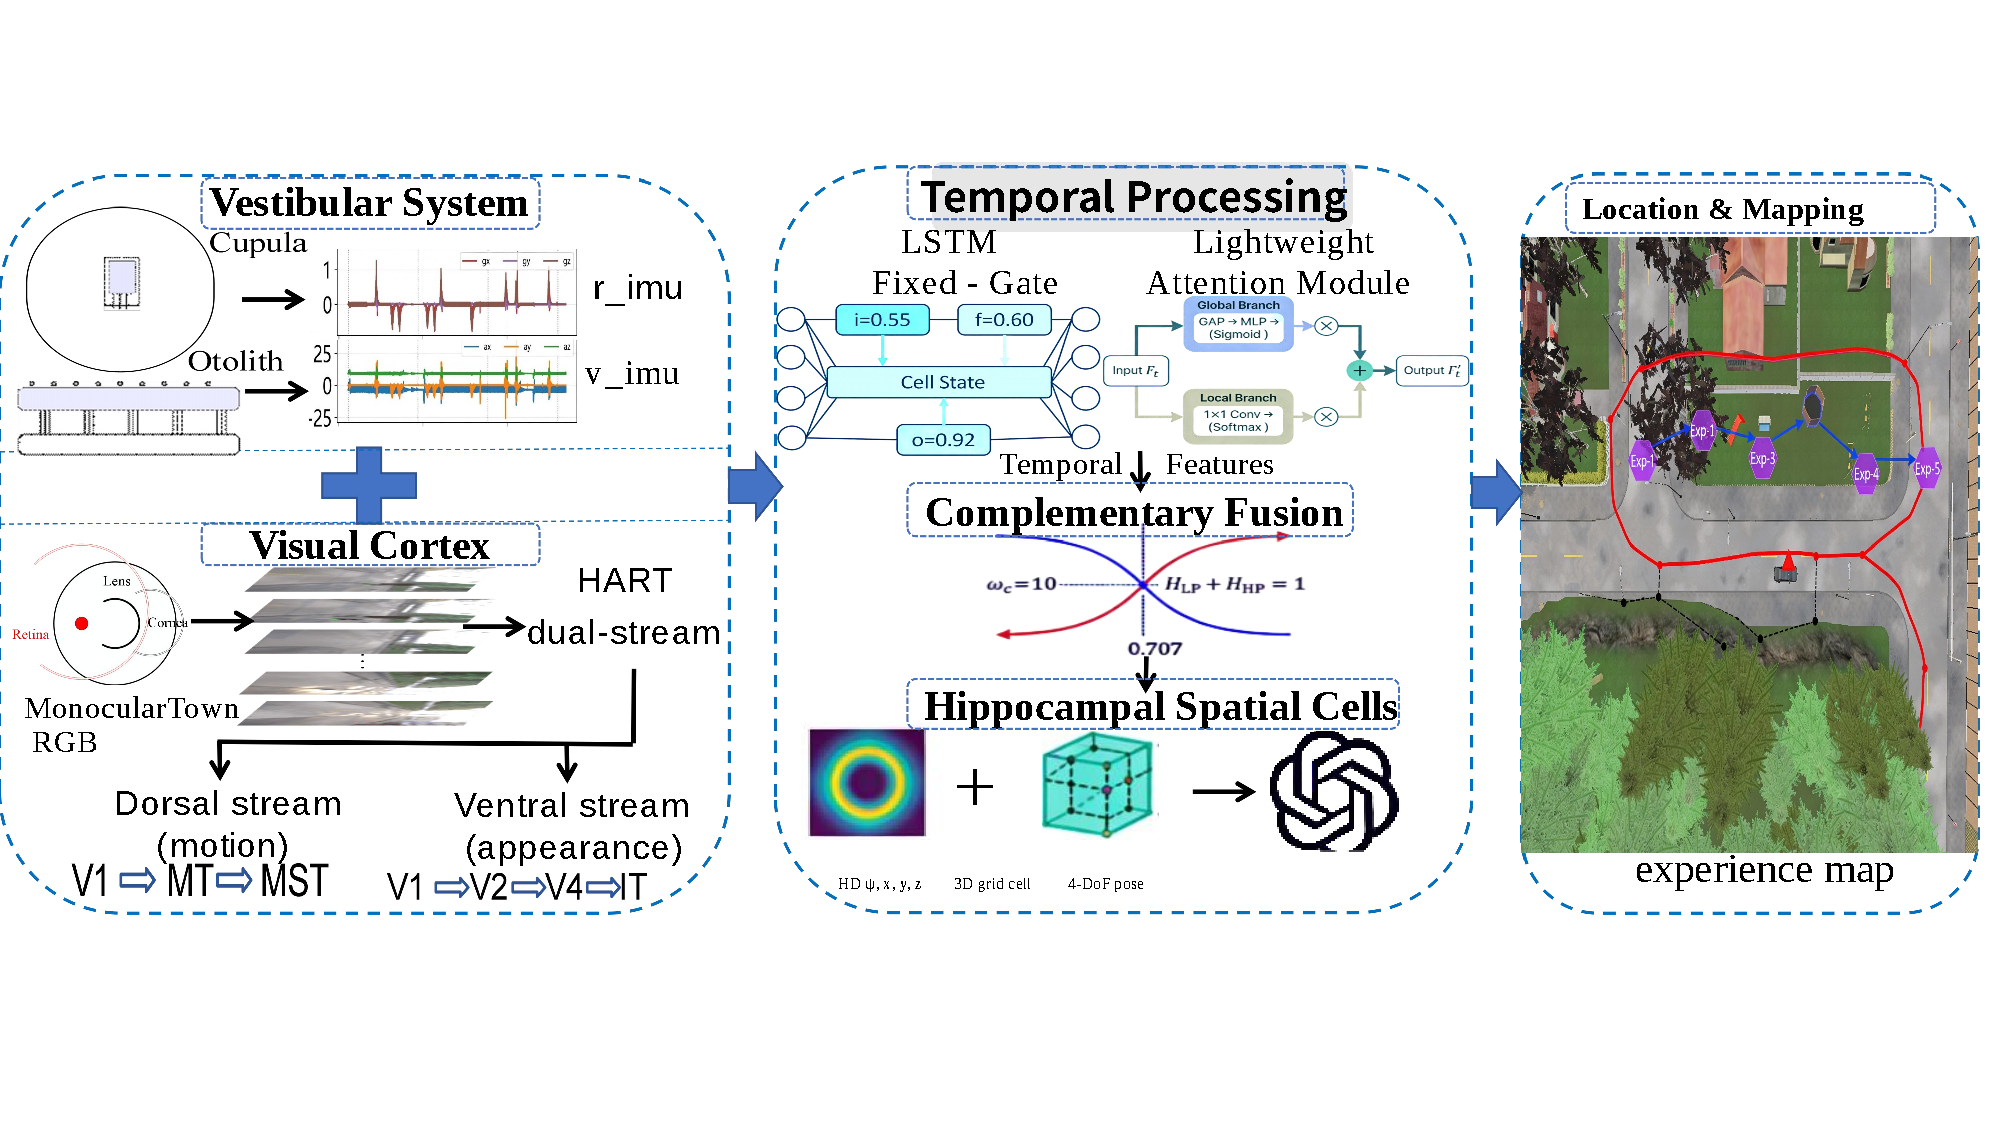
\includegraphics[trim=0pt 97pt 6pt 82pt, clip, width=0.95\textwidth]{fig/2_framework.pdf}
    \caption{Self-contained end-to-end data flow of the proposed multimodal visual-inertial framework. Raw inputs are monocular RGB images and IMU measurements. The visual module splits signals into scene recognition and motion estimation branches; the vestibular module outputs high-frequency inertial motion. Two modalities are fused with the frequency-domain principle of Section~\ref{sec:principle}, instantiated as a fixed-dimension (10-state) EKF. The fused kinematics drive the spatial network to update the unified 4-DoF global state $\mathbf{X}_t$ defined in Eq. \eqref{eq:global_state}. The experience graph module performs loop relaxation to eliminate long-term trajectory drift. All submodules share the standardized state-space variables proposed in this section.}
    \label{fig:system_overview}
\end{figure*}
This work designs a multimodal visual-inertial signal processing system for robot localization, which consists of three tightly coupled functional subsystems: hierarchical multi-scale visual feature operator, vestibular-inertial sensor state estimator, and metric spatial state encoding network. Unlike tightly coupled visual-inertial estimators that augment the state with feature clones, the proposed system keeps a state of fixed dimension and makes the frequency-domain complementarity of the two modalities explicit: the inertial channel supplies the high-frequency prediction, the visual channel supplies gated low-frequency corrections, and the resulting metric state is integrated by a continuous attractor spatial network that suppresses long-term trajectory drift.

\subsubsection{Global Discrete State-Space Model}
To provide a unified mathematical foundation for all subsequent submodule derivations, we first define the discrete state-space representation of the system at time $t$.

1) Multimodal raw input vector
\begin{equation}
    \mathbf{U}_t = \left[ I_t,\, \mathbf{a}_t^\top,\, \boldsymbol{\omega}_t^\top \right]
    \label{eq:input_vec}
\end{equation}
where $I_t$ denotes the captured monocular RGB image; $\mathbf{a}_t$ and $\boldsymbol{\omega}_t$ stand for accelerometer linear acceleration and gyroscope angular velocity measurements, respectively.

2) Core 4-DoF global pose state vector
\begin{equation}
    \mathbf{X}_t = \left[ x_t,\, y_t,\, z_t,\, \psi_t \right]^\top \in \mathbb{R}^3 \times \mathrm{SO}(2)
    \label{eq:global_state}
\end{equation}
In this formulation, $(x_t, y_t, z_t) \in \mathbb{R}^3$ represent global 3D translational coordinates (unit: meter), and $\psi_t \in [-\pi,\pi)$ denotes horizontal yaw angle (unit: radian).

3) Unified state evolution mapping function
\begin{equation}
    \mathbf{X}_{t+1} = \mathcal{F}\big(\mathbf{X}_t,\, \mathbf{U}_t\big)
    \label{eq:state_evolution}
\end{equation}
The mapping $\mathcal{F}(\cdot)$ encapsulates the complete forward pipeline, including multi-scale visual feature extraction, inertial motion calculation, frequency-domain multimodal fusion and spatial network path integration. Detailed mathematical decomposition of $\mathcal{F}(\cdot)$ is presented in Sections~\ref{sec:visual_cortex}--\ref{sec:fusion} (visual cortex, vestibular system, and complementary fusion) and Sections~\ref{sec:scale_recovery}--\ref{sec:loop_closure} (scale recovery and the spatial memory system).

As visualized in Fig.~\ref{fig:system_overview}, the end-to-end data pipeline consists of five sequential coupled modules:
1. Hierarchical dual-stream visual front-end: Parallel ventral/dorsal branches are constructed to independently generate scene descriptors and compute pixel-wise ego-motion, eliminating mutual interference between recognition and tracking tasks.
2. Vestibular IMU processing module: Derives high-frequency transient motion signals from raw inertial data without iterative online bias calibration.
3. Complementary fusion unit: Adopts first-order IIR filters to separate low-frequency visual drift and high-frequency inertial noise, outputting smoothed translational and rotational kinematics.
4. Metric spatial encoding network: Updates distributed spatial cell states using fused motion cues, and suppresses integral drift via visual template anchoring constraints.
5. Topological experience graph: Records historical visual descriptors and spatial cell snapshots, and executes global graph relaxation once loop closures are detected to guarantee globally consistent metric poses.

\noindent Above this five-module pipeline, the deployed system adds two higher-level corrections that operate on the fused estimate rather than on the raw sensor streams: a monocular scale recovery branch (Section~\ref{sec:scale_recovery}) that drives the EKF's scale state from a lightweight, train-once head over a frozen depth foundation model, and a learned-embedding loop-closure line (Section~\ref{sec:loop_closure}) that re-anchors the trajectory at verified revisits. Both are trained once on simulated data and frozen at deployment --- in contrast to the baseline's kinematic scale observability, which plateaus at the VO-relative scale and recovers no absolute scale. Together they turn the tracking core from an up-to-scale VIO estimator into the metric-scale system evaluated in the experiments.

\subsection{Visual Cortex: Ventral and Dorsal Pathways}
\label{sec:visual_cortex}

The visual front-end --- neuroanatomically, the dual ventral (``what'') and dorsal (``where'') streams of the visual cortex --- implements a biologically-plausible processing pipeline inspired by the hierarchical architecture of the primate visual cortex, transforming raw RGB images into compact scene descriptors suitable for place recognition and motion estimation.

\textbf{Hierarchical Feature Extraction.} Given an RGB image $I_t\in\mathbb{R}^{H\times W\times 3}$, we define a sequence of operators that mimic processing stages from retina through inferotemporal cortex.

\textbf{Stage 1: Retinal and LGN Processing.} The initial preprocessing simulates early visual processing in the retina and lateral geniculate nucleus (LGN):
\begin{align}
     & \text{Luminance channel:}\quad Y_t = \mathcal{G}(I_t) = 0.299R+0.587G+0.114B              \\
     & \text{Local contrast enhancement:}\quad U_t = \mathcal{C}_\lambda(Y_t),\quad \lambda=0.02 \\
     & \text{Receptive field simulation:}\quad V_t = U_t * \mathcal{K}_\sigma,\quad \sigma=0.5
\end{align}
where $\mathcal{G}$ is the grayscale conversion operator, $\mathcal{C}_\lambda$ is CLAHE (Contrast Limited Adaptive Histogram Equalization) with clip limit $\lambda$, and $\mathcal{K}_\sigma$ is a Gaussian kernel with standard deviation $\sigma$. CLAHE adaptively enhances local contrast while preventing over-amplification of noise, mimicking the center-surround antagonistic organization of retinal ganglion cells.

\textbf{Stage 2: Primary Visual Cortex (V1-V4) Processing.} Mid-level processing normalizes and standardizes the representation:
\begin{align}
     & \text{Dynamic range normalization:}\quad \tilde V_t = \frac{V_t-\min(V_t)}{\max(V_t)-\min(V_t)}     \\
     & \text{Spatial standardization:}\quad Z_t = \mathcal{D}(\tilde V_t)\in\mathbb{R}^{12\times16}        \\
     & \text{Global mean subtraction:}\quad Z_t(i,j)\leftarrow Z_t(i,j)-\frac{1}{192}\sum_{k=1}^{12}\sum_{l=1}^{16}Z_t(k,l)
\end{align}
where $\mathcal{D}$ is the downsampling operator (bilinear interpolation). Global mean subtraction removes overall intensity variations while preserving spatial structure, analogous to divisive normalization in V1 and V2.

\textbf{Stage 3: Inferotemporal (IT) Representation.} The final representation is a compact vectorized descriptor:
\begin{equation}
    \boldsymbol{\phi}_t=\mathrm{vec}(Z_t)\in\mathbb{R}^{192}
\end{equation}
where $\mathrm{vec}(\cdot)$ denotes vectorization operator mapping 2D feature map to one-dimensional descriptor, and $\boldsymbol{\phi}_t$ is holistic scene feature vector at timestamp $t$.
This $12 \times 16 = 192$-dimensional feature vector serves as a holistic scene descriptor analogous to the view-selective, position-invariant representations in IT cortex.

\textbf{Visual Template Matching and Place Recognition.} Place recognition is achieved through template matching using cosine similarity, which is more robust than intensity-based metrics like sum-of-absolute-differences (SAD):
\begin{equation}
    d_{\cos}(\boldsymbol{\phi}_t,\boldsymbol{\phi}_i)=1-\frac{\boldsymbol{\phi}_t^\top\boldsymbol{\phi}_i}{\lVert\boldsymbol{\phi}_t\rVert\,\lVert\boldsymbol{\phi}_i\rVert}
\end{equation}
A new visual template (VT) is created when the current scene is sufficiently different from all existing templates:
\begin{equation}
    \text{Create new VT if }\min_{i \in \mathcal{VT}} d_{\cos}(\boldsymbol{\phi}_t, \boldsymbol{\phi}_i)>\tau_{vt},\quad \tau_{vt}=0.08
\end{equation}
The threshold $\tau_{vt}=0.08$ is significantly lower than the traditional value (0.15 in OpenRatSLAM), enabling finer discrimination between similar scenes. Experimental validation shows this results in up to 39$\times$ increase in template count (from 5 to 195 templates in urban environments), providing much richer place representation.

\textbf{Dual-Stream Architecture and Bio-Inspired Temporal Modeling.} Building upon the hierarchical feature extraction described above, our visual processing incorporates two key bio-inspired innovations: (1) dual-stream architecture mimicking ventral/dorsal path\-ways, and (2) fixed-gate LSTM for temporal coherence without training data requirements.

\textbf{Dual-Stream Visual Processing.}
Following the dual-stream theory of biological vision~\cite{Goodale1992, Mishkin1983}, we explicitly model two parallel processing path\-ways from V1 outputs:

\textbf{Oriented-Gradient Channel} (spatial-layout branch, V1$\rightarrow$V4): Processes spatial location and appearance structure through gradient-based features:
\begin{equation}
    \mathbf{F}^{\text{grad}}_t = 0.6 \cdot \|\nabla Z_t\| + 0.4 \cdot Z_t
\end{equation}
where $\|\nabla Z_t\|$ is the gradient magnitude computed via Sobel operators, capturing edge orientation analogous to orientation-selective V4 responses. The channel implements the V1$\rightarrow$V4 stage of the hierarchy: the gradient magnitude plays the role of the orientation-selective responses of V1 simple cells, and the weighted sum aggregates them into a compact spatial-layout map that feeds the temporal model. The weights $0.6/0.4$ are fixed heuristic constants chosen once at implementation and shared by all scenes; the gradient term dominates because edge structure carries the spatial-layout evidence.

\textbf{Ventral Channel} (``what'' pathway, V1$\rightarrow$V4$\rightarrow$IT): Processes object identity and scene features through texture and contrast:
\begin{equation}
    \mathbf{F}^{\text{ventral}}_t = 0.4 \cdot Z_t + 0.3 \cdot \sigma_{\text{local}}(Z_t) + 0.3 \cdot \mathcal{C}_\lambda(Z_t)
\end{equation}
where $\sigma_{\text{local}}$ computes local standard deviation (texture features) and $\mathcal{C}_\lambda$ provides contrast enhancement, mimicking V4's selectivity for complex features and IT's invariant object representations.

The dual streams are then integrated through a lightweight global-local feature modulation mechanism that approximates self-attention effects using global statistics rather than full Query-Key-Value operations, maintaining $\mathcal{O}(N)$ complexity for real-time per\-for\-mance.

\textbf{Fixed-Gate LSTM for Zero-Shot Temporal Modeling.}
Unlike conventional data-driven LSTMs that require extensive training on do\-main-spe\-cif\-ic datasets, our temporal module employs manually-tuned fixed gate values inspired by biological ves\-tib\-u\-lar-visual integration principles~\cite{Angelaki2004, Cullen2012}:
\begin{align}
    \text{Input gate: }  & i_t = 0.5 \quad \text{(controls new information intake)} \\
    \text{Forget gate: } & f_t = 0.5 \quad \text{(retains 50\% historical context)} \\
    \text{Output gate: } & o_t = 0.9 \quad \text{(emphasizes current perception)}
\end{align}
where $i_t$, $f_t$, $o_t$ represent fixed input gate, forget gate, output gate of bio-inspired LSTM module, respectively.


This design offers three critical advantages for SLAM applications:

\textbf{(1) Zero-shot deployment capability:} No training data required, enabling immediate deployment in novel environments. This is crucial for SLAM where each environment presents unique visual characteristics and collecting representative training data is impractical. Our validation across six diverse scenarios (urban, highway, indoor) without any environment-specific tuning demonstrates robust generalization.

\textbf{(2) Biological interpretability:} Gate values reflect em\-pir\-i\-cal\-ly-val\-i\-dat\-ed principles from neuroscience. The forget gate ($f_t=0.5$) implements short-term spatial memory retention consistent with hippocampal replay dynamics, where recent experiences are preferentially retained for path integration. The high output gate ($o_t=0.9$) prioritizes current sensory input, mimicking the ves\-tib\-u\-lar system's emphasis on immediate self-motion cues for balance and navigation. The moderate input gate ($i_t=0.5$) balances novelty detection with stability.

\textbf{(3) Computational efficiency:} Eliminates training overhead (no backpropagation, no gradient computation) while maintaining real-time per\-for\-mance (39--76~FPS, MATLAB reference implementation, CPU). Fixed gates can be directly implemented in hardware (e.g., FPGAs, neuromorphic chips) without weight storage or update logic, enabling deployment on resource-constrained platforms.

The LSTM processes fused gradient-ventral features sequentially, maintaining hidden state $\mathbf{H}_t$ and cell state $\mathbf{C}_t$ across timesteps:
\begin{align}
    \mathbf{C}_t & = f_t \odot \mathbf{C}_{t-1} + i_t \odot \tanh(\mathbf{F}^{\text{fused}}_t) \\
    \mathbf{H}_t & = o_t \odot \tanh(\mathbf{C}_t)
\end{align}
where $\odot$ denotes element-wise Hadamard product, $\mathbf{C}_t$ is the LSTM cell state, $\mathbf{H}_t$ is the temporal hidden state, and $\mathbf{F}^{\text{fused}}_t$ integrates the oriented-gradient and ventral appearance features.

\textbf{Comparison with Learning-Based Approaches.} Section~\ref{sec:experiments} demonstrates that our fixed-gate LSTM achieves comparable or superior per\-for\-mance to NeuroSLAM's learned LSTM (55\% improvement in RMSE) while offering zero-shot deployment. This validates that principled bio-inspired design can match or exceed data-driven learning when the underlying task structure aligns with biological mechanisms---in this case, spatial navigation where biological systems have evolved highly optimized solutions over millions of years.

\textbf{Visual Motion Extraction.} In addition to scene recognition, the visual front-end extracts ego-motion cues from inter-frame feature correspondences, mimicking the dorsal stream processing in area MST (medial superior temporal).

\textbf{Sparse Feature Correspondence.} Let $\mathbf{K}\in\mathbb{R}^{3\times 3}$ be the camera intrinsic matrix. Each frame is described by $N$ ORB keypoints ($N{=}2000$) with rotated-BRIEF descriptors; putative correspondences are established by k-nearest-neighbour matching with the Lowe ratio test ($k{=}2$, ratio $0.7$). Matched points are normalized to camera coordinates:
\begin{equation}
    \tilde{\mathbf{q}}_i^t = \mathbf{K}^{-1}\begin{bmatrix}\mathbf{p}_i^t\\ 1\end{bmatrix},\qquad \mathbf{q}_i^t = \pi(\tilde{\mathbf{q}}_i^t)=\frac{1}{\tilde{q}_{i,3}^t}\begin{bmatrix}\tilde{q}_{i,1}^t\\ \tilde{q}_{i,2}^t\end{bmatrix}
\end{equation}
where $\pi$ is perspective projection.

\textbf{Rotation--Translation Estimation.} The normalized correspondences $\{(\mathbf{q}_i^{t-1},\,\mathbf{q}_i^{t})\}$ satisfy the epipolar constraint
\begin{equation}
    {\mathbf{q}_i^{t}}^{\top}\,\mathbf{E}\,\mathbf{q}_i^{t-1}=0,\qquad \mathbf{E}=[\mathbf{t}]_{\times}\mathbf{R},
\end{equation}
where $\mathbf{E}$ is the essential matrix and $[\mathbf{t}]_{\times}$ the skew-symmetric matrix of the translation vector. $\mathbf{E}$ is estimated by a RANSAC-wrapped minimal solver (confidence $0.999$, inlier threshold $1.0$~px) and decomposed via $\mathrm{recoverPose}$ into the inter-frame rotation $\mathbf{R}$ and the translation direction. Robustness is enforced at two levels: descriptor-level uniqueness (Lowe ratio test) and geometric-level consensus (the RANSAC consensus set). The visual yaw rate $r_t^{\mathrm{vis}}$ is extracted from the ZYX Euler decomposition of $\mathbf{R}$ (with a gimbal-lock guard); the translation is returned as a unit-norm direction $\hat{\mathbf{t}}$ --- monocular decomposition determines the direction only, never the magnitude.

\textbf{Scale Ambiguity and Observation Injection.} Because $\hat{\mathbf{t}}_t$ is unit-norm, the decomposition carries no metric magnitude: the metric displacement over one inter-frame interval is $\Delta\mathbf{p}^{\mathrm{vis}}_t = s_t\,\hat{\mathbf{t}}_t$, where $s_t = \exp(\log s_t)$ is the online scale state maintained by the EKF (Section~\ref{sec:scale_recovery}), expressed in metres per unit VO displacement; a single symbol $s$ is used for this quantity throughout. The EKF converts this displacement into a velocity over the true inter-update interval (Section 4.1). The inlier consensus doubles as a degeneracy gate: below 20 correspondences the frame is treated as degenerate and is not treated as a reliable motion measurement; the zero-displacement placeholder returned by the front-end enters the filter with its observation noise inflated by the same quality factor, so it acts as a no-motion prior rather than as an independent velocity measurement. Otherwise the inlier count $n_{\mathrm{inl}}$ maps to a quality factor $q_f=\clip(60/n_{\mathrm{inl}},\,1/3,\,3)$ --- $q_f{=}1$ at 60 inliers, $q_f{=}3$ at 20, and $q_f$ saturating at $1/3$ when the count exceeds 180 --- which multiplies the EKF observation covariance together with a smooth residual factor and is clamped to $[0.008,10]$ (Section~\ref{sec:deployed_filter}).

Beyond this motion stream, the visual front-end also provides the pixel-level metric depth field $\hat z_t$ (frozen DAv2 backbone) and the learned scene embeddings $\boldsymbol{e}_t$ consumed by the two higher-level corrections (Section~\ref{sec:scale_recovery}); the motion pathway above never consumes depth --- $\hat z_t$ and $\boldsymbol{e}_t$ are inferred asynchronously and cached, entering only the scale branch and the loop-closure line, outside the real-time critical path.

\subsection{Vestibular System}
\label{sec:vestibular}

The vestibular front-end processes inertial measurements to extract self-motion cues analogous to the mammalian ves\-tib\-u\-lar system. The ves\-tib\-u\-lar apparatus comprises semicircular canals (angular velocity) and otolith organs (linear acceleration).

\textbf{Angular Velocity Extraction.} From the gyroscope measurements $\mathbf{g}_t\in\mathbb{R}^3$ (IMU frame), we use the raw $z$-axis gyro. A constant bias is estimated once from the static start-up window and subtracted thereafter (Section~\ref{sec:fusion}); no per-frame bias estimation is performed. For 4-DoF lo\-cal\-i\-za\-tion-and-map\-ping under a planar constraint, the yaw (azimuthal) angular velocity is approximated by
\begin{equation}
    r_t \approx \mathbf{e}_z^\top\,\boldsymbol{\omega}_t^g,\quad \mathbf{e}_z=(0,0,1)^\top.
\end{equation}
where $\boldsymbol{\omega}_t^g$ is raw gyroscope angular velocity vector measured by IMU, and $\mathbf{e}_z$ is unit vertical basis vector.
This corresponds to the horizontal semicircular canal cue, adequate for our complementary fusion with vision.

\textbf{Linear Acceleration Usage (Simplified).} We adopt a lightweight approximation consistent with the codebase: using the accelerometer magnitude and the $z$-axis reading with a constant gravity subtraction $g\!=\!9.81$ to derive indicative translational and vertical velocity components over the frame interval $\Delta t$:
\begin{align}
    v^\mathrm{imu}_{trans}(t) & \approx \max\big(0, (\lVert\mathbf{a}_t\rVert - g)\,\Delta t\,k_t\big), \\
    v^\mathrm{imu}_{z}(t)     & \approx (a_{t,z} - g)\,\Delta t\,k_z,
\end{align}
where $g=9.81\,\mathrm{m/s^2}$ is gravitational acceleration, $k_t, k_z$ are constant scaling gains matching our implementation constants, and $\Delta t$ denotes the frame sampling interval. This cue carries no bias or gravity-vector state and provides the high-frequency channel of the reference implementation (Section~\ref{sec:reference_impl}); the deployed filter obtains the same high-frequency information from the IMU propagation of Section~\ref{sec:deployed_filter}, not from this heuristic.

\textbf{Bias Estimation.} The accelerometer and gyroscope biases that enter the kinematic cues are estimated once, in the static start-up window of each sequence (the first 200 samples with the platform at rest), and are then held constant; no online gravity-vector estimation is performed and a constant gravity magnitude is used for specific-force compensation. This keeps the front-end free of extra filter states and is sufficient at the 20\,Hz CARLA cadence (KITTI~07 is processed at its native $\approx$9.6\,Hz, $\Delta t\approx0.104$\,s); the residual effect of a fixed gravity magnitude is analysed as a failure mode in the discussion.

\subsection{Vestibular--Visual Fusion: Frequency-Domain Principle and Deployed Filter}
\label{sec:fusion}

\textbf{How NeuroLocMap operates.} The modules of the framework are coupled in one direction only, so the operating chain can be stated before the equations. For every camera frame $t$: (1) the visual front-end returns a relative displacement, a yaw increment and an inlier count; (2) the filter is propagated IMU-step by IMU-step across the inter-frame interval with \eqref{eq:ekf_pred}--\eqref{eq:ekf_cov}; (3) the gated corrections of Table~\ref{tab:gates} are applied in a fixed order --- velocity amplitude, attitude, scale, position --- because each branch supplies a quantity that a later one consumes (the position anchor is expressed in metres through the scale state, and the velocity amplitude is compared in the same units); the heading branch of the table is implemented but disabled in the configuration that produced all reported numbers, and the chain above therefore runs on four active branches; (4) the filtered pose is published and, in EKF-odometry mode, handed to the spatial layer as its motion source; (5) the grid-cell attractor integrates the frame-to-frame displacement into a bump of activity and the head-direction layer carries the yaw (Section~\ref{sec:grid_cells}); (6) when the current visual template and spatial code are novel, an experience node is created and linked to its predecessor (Section~\ref{sec:loop_closure}); (7) an accepted loop-closure event relaxes a drift field over the stored trajectory and re-anchors the path integrator. Steps (1)--(4) constitute the filter; steps (5)--(7) act on its output and never write back into it.

Three design choices make this chain work. First, the frequency split assigns each modality the band in which it is reliable, so the filter never has to arbitrate between two equally trusted absolute observations. Second, the state dimension is fixed at ten, so the cost per update does not grow with the number of tracked features and any single branch can be switched off without perturbing the others (Section~\ref{sec:deployed_filter}). Third, every higher-level correction acts downstream, on the output trajectory, which keeps the ablation of Section~\ref{sec:ablation} causal: a difference between two configurations is attributable to the module that was removed. Sections~\ref{sec:scale_recovery}--\ref{sec:loop_closure} specify steps (3)--(7) of this chain, each in the same order: what enters, what is computed, what leaves.

Visual and inertial modalities provide complementary information: visual odometry yields accurate low-frequency motion estimates but drifts over long horizons, whereas IMU integration provides reliable high-frequency motion cues but accumulates bias drift. Exploiting this frequency-domain separation permits robust fusion without joint nonlinear optimization over visual features. The framework carries this principle in two clearly separated forms. The MATLAB reference implementation realizes it directly, as a fixed-weight convex combination of complementary low- and high-pass channels (Section~\ref{sec:reference_impl}). The deployed system realizes it as a loosely coupled EKF of fixed state dimension, in which the inertial channel supplies the high-frequency prediction and the visual channel supplies low-frequency, gated corrections. All results reported in this paper are produced by the deployed filter; the fixed-weight combination is retained only as an ablation reference and as the object of the per-module runtime measurements. Figure~\ref{fig:imu_visual_fusion} illustrates the frequency-domain characteristics of the principle and its biological analogue in ves\-tib\-u\-lar--visual integration.

\begin{figure*}[!t]
    \centering
    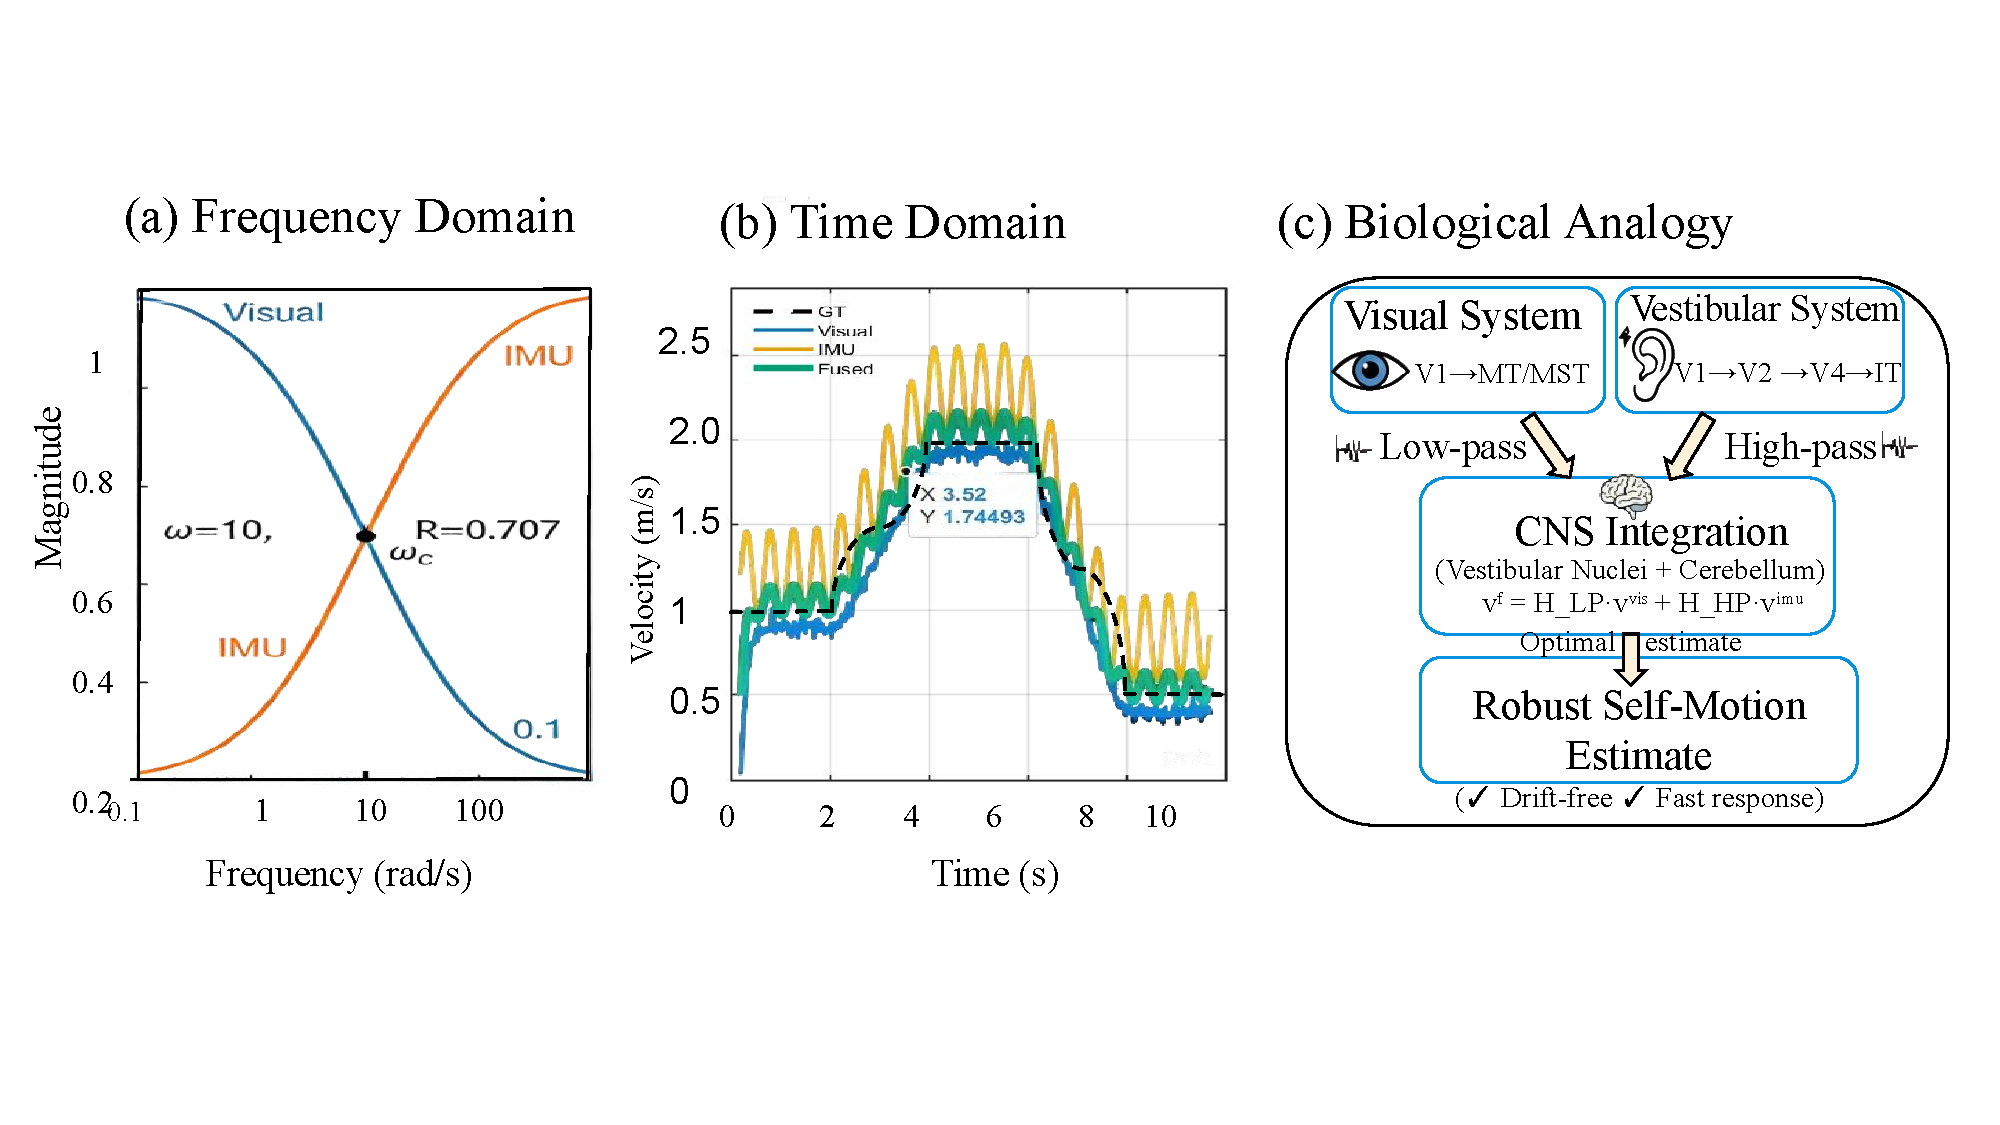
\includegraphics[trim=12pt 107pt 20pt 98pt, clip, width=\textwidth]{fig/imu_visual_complementary_fusion.pdf}
    \caption{Frequency-domain principle of the vestibular--visual fusion. (a) Frequency-domain analysis of the complementary low- and high-pass characteristics. (b) Time-domain signal comparison. (c) Biological analogy to ves\-tib\-u\-lar--visual integration in the CNS. (a)--(c) illustrate the principle of Section~\ref{sec:principle}; the deployed filter that produces all reported results is specified in Section~\ref{sec:deployed_filter}.}
    \label{fig:imu_visual_fusion}
\end{figure*}

\subsubsection{Biological Principle and Frequency-Domain Complementarity}
\label{sec:principle}

\textbf{Filter Design.} Let $\mathcal{L}_\tau$ denote a low-pass filter with time constant $\tau$, and $\mathcal{H}_\tau$ the complementary high-pass filter satisfying $\mathcal{L}_\tau+\mathcal{H}_\tau=\mathrm{Id}$, with $\mathrm{Id}$ the identity operator. Realized recursively,
\begin{equation}
    L_t = \alpha L_{t-1} + (1-\alpha) x_t,\qquad L_0=0 \label{eq:lowpass}
\end{equation}
\begin{equation}
    H_t = x_t - L_t \label{eq:highpass}
\end{equation}
where $\alpha$ is the IIR forgetting factor, $L_t$ the low-frequency smoothed signal, and $H_t$ its residual high-frequency component.

\textbf{Biological Analogy.} This is the discrete counterpart of multisensory integration in the ves\-tib\-u\-lar nuclei and posterior parietal cortex (area~7a), where visual and ves\-tib\-u\-lar signals are combined to estimate self-motion; neurons in these regions exhibit weighted combinations of the two tuning profiles, with dynamic weighting according to signal reliability.

\textbf{Discrete-Time Implementation.} With sampling interval $\Delta t$ we implement first-order IIR filters and set the forgetting factors from the target time constants, $\alpha=\exp(-\Delta t/\tau)$ and $\alpha_r=\exp(-\Delta t/\tau_r)$, so that the analogue cut-off is reproduced at the 20\,Hz cadence used here.

\textbf{Frequency-Domain Transfer Functions.} In the Laplace domain with $s=j\omega$,
\begin{equation}
    H_{LP}(s) = \frac{1}{1+\tau s} = \frac{1/\tau}{s+1/\tau}, \label{eq:h_lp}
\end{equation}
\begin{equation}
    H_{HP}(s) = \frac{\tau s}{1+\tau s} = \frac{s}{s+1/\tau}, \label{eq:h_hp}
\end{equation}
satisfying $H_{LP}(s)+H_{HP}(s)=1$ (unity gain at all frequencies). The cut-off $\omega_c=1/\tau$ separates the two regions: for $\omega\ll\omega_c$, $|H_{LP}|\approx1$ and $|H_{HP}|\approx0$, so the visual pathway dominates (drift-free, slower dynamics); for $\omega\gg\omega_c$ the IMU cues dominate (fast but drifting). With $\tau=0.1$\,s the cut-off is $\omega_c=10$\,rad/s ($\approx1.6$\,Hz), so that IMU handles high-frequency motion ($>2$\,Hz: vibration, rapid turns) while vision corrects low-frequency drift ($<1$\,Hz). This mimics ves\-tib\-u\-lar--visual integration, where ves\-tib\-u\-lar organs respond in 0.1--10\,Hz and visual motion perception dominates below 0.5\,Hz~\cite{Angelaki2004}.

\subsubsection{Temporal Alignment}
\label{sec:alignment}

In the CARLA synchronous acquisition setting (20\,Hz, $\Delta t=0.05$\,s) both sensors are driven by a single cadence, and a lightweight aligner pairs each camera frame with the nearest IMU sample within a 0.02\,s tolerance using greedy one-to-one matching (each IMU sample is consumed at most once). Timestamps of the aligned streams were checked frame by frame over all 5000 CARLA frames and the 1101 KITTI~07 frames, with no gaps and no dropped frames, so the fusion operates on pre-aligned samples and requires no intra-frame interpolation.

\subsubsection{Deployed Implementation: Total-State EKF with Error-State Covariance}
\label{sec:deployed_filter}

\textbf{State.} The deployed fusion core is a total-state EKF whose covariance is propagated in error-state form, with state
\begin{equation}
    \mathbf{x}_t=\big[x,y,z,\ v_x,v_y,v_z,\ \phi,\theta,\psi,\ \log s_t\big]^{\!\top}
    \label{eq:state}
\end{equation}
i.e.\ position, velocity, Euler attitude and a tenth state $\log s_t$, the online scale that links the VO frame to the metric world (notation of Section~\ref{sec:notation}; the scale branch is detailed in Section~\ref{sec:scale_recovery}). The tenth state is what makes the other nine interpretable in metres: without it the visual channel would only be consistent up to scale.

\textbf{Prediction.} Between observations the state is propagated by IMU kinematics,
\begin{equation}
\begin{aligned}
    \mathbf{a}^{w}_t &= R(\boldsymbol{\Theta}_t)\big(\mathbf{a}_t-\mathbf{b}_a\big)+\mathbf{g}_w,\qquad \mathbf{g}_w=[0,0,-g]^{\top},\\
    \boldsymbol{\Theta}_{t+1} &= \wrap\big(\boldsymbol{\Theta}_t+(\boldsymbol{\omega}_t-\mathbf{b}_g)\Delta t\big),\\
    \big(v^{x}_{t+1},v^{y}_{t+1}\big) &= \big(v^{x}_t,v^{y}_t\big)+\big(a^{w,x}_t,a^{w,y}_t\big)\Delta t,\qquad v^{z}_{t+1}=0,\\
    \big(p^{x}_{t+1},p^{y}_{t+1}\big) &= \big(p^{x}_t,p^{y}_t\big)+\big(v^{x}_t,v^{y}_t\big)\Delta t,\qquad z_{t+1}=z_t,
\end{aligned}
    \label{eq:ekf_pred}
\end{equation}
with $R(\cdot)$ the body-to-world rotation, $\wrap(\cdot)$ mapping an angle to $(-\pi,\pi]$, $g$ constant, and $\mathbf{b}_a,\mathbf{b}_g$ fixed from the static start (Section~\ref{sec:vestibular}). Three properties of this form are deliberate rather than incidental. (i) The vertical channel is \emph{frozen}: the vertical velocity is clamped to zero after every prediction and the altitude is held at its initial value, so the filter propagates exactly the planar 4-DoF motion model assumed in Section~\ref{sec:framework_arch} --- this clamp is the implementation of the 4-DoF assumption, and it is what keeps the planar VO increments and the tenth scale state mutually consistent. (ii) Integration is explicit in the current velocity; no $\tfrac12\mathbf{a}\Delta t^{2}$ term is used, so the position Jacobian contains only $\partial p^{x}/\partial v^{x}=\partial p^{y}/\partial v^{y}=\Delta t$ and the attitude block of $\mathbf{F}$ is the identity, which keeps the Jacobian sparse and cheap to form. (iii) The attitude is propagated with the gyroscope only; the visual attitude branch of Table~\ref{tab:gates} corrects it downstream. The covariance follows
\begin{equation}
    \mathbf{P}_{t+1}=\mathbf{F}_t\mathbf{P}_t\mathbf{F}_t^{\top}+\mathbf{Q}_c\,\Delta t,
    \label{eq:ekf_cov}
\end{equation}
with process noise and initial covariance fixed once for all sequences,
\begin{equation}
\begin{aligned}
    \mathbf{Q}_c&=\mathrm{diag}\big(0.18,0.18,0.09,\ 0.72,0.72,0.36,\\
    &\qquad\qquad 7.2\mathrm{e}{-3},7.2\mathrm{e}{-3},1.8\mathrm{e}{-2},\ 2.0\mathrm{e}{-5}\big),\\
    \mathbf{P}_0&=\mathrm{diag}\big(2,2,0.5,\ 2,2,1,\ 0.05,0.05,0.05,\ 0.64\big),
\end{aligned}
\end{equation}
ordered as $(p,v,\Theta,\log s)$: the entries of $\mathbf{Q}_c$ carry the units $\mathrm{m^2\,s^{-1}}$, $\mathrm{m^2\,s^{-3}}$, $\mathrm{rad^2\,s^{-1}}$ and $\mathrm{s^{-1}}$ (the tenth state is $\log s$, dimensionless, so its noise density is per second), and those of $\mathbf{P}_0$ the units $\mathrm{m^2}$, $\mathrm{m^2\,s^{-2}}$, $\mathrm{rad^2}$ and $1$; the scale variance $0.64$ corresponds to the $\sigma_0=0.8$ log prior, and $\log s$ starts at $0$ (unit scale). A pure-IMU dead-reckoning copy is maintained in parallel for diagnostic purposes; it is not used as a comparison row in the experiments.

\textbf{Gated Observation Update.} Each branch produces an innovation $\mathbf{y}=\mathbf{z}-h(\hat{\mathbf{x}})$ with $\mathbf{S}=\mathbf{H}\mathbf{P}\mathbf{H}^{\top}+\mathbf{R}$, accepted only if
\begin{equation}
    \mathbf{y}^{\top}\mathbf{S}^{-1}\mathbf{y}<\chi^2(d;\alpha),
    \label{eq:gate}
\end{equation}
and applied in the Joseph form, which preserves symmetry and positive definiteness:
\begin{equation}
    \mathbf{P}^{+}=(\mathbf{I}-\mathbf{K}\mathbf{H})\mathbf{P}(\mathbf{I}-\mathbf{K}\mathbf{H})^{\top}+\mathbf{K}\mathbf{R}\mathbf{K}^{\top},
    \quad \mathbf{K}=\mathbf{P}\mathbf{H}^{\top}\mathbf{S}^{-1}.
    \label{eq:joseph}
\end{equation}

The branches, their models and the deployed thresholds are listed in Table~\ref{tab:gates}, and they are applied in the order of the table for the dependency reason given above. Branch~1 (disabled in the deployed runs, Table~\ref{tab:gates}) would recover yaw from turn kinematics: on frames with mean speed $>3$\,m/s, $|a_\perp|>0.3$\,m/s$^2$ and $|\omega_z|<1.2$\,rad/s, the ratio $a_\perp/|v|$ is integrated onto a heading base that is independent of both the gyroscope and the current heading estimate, giving a yaw-angle observation with a per-frame step limit of 0.26\,rad ($\approx15^{\circ}$). Branch~4 is a dual-path, log-domain scale observation: the calibrated depth scale of Section~\ref{sec:scale_recovery} takes precedence and is frozen inside a 0.30 dead band in the log domain ($\approx1.35\times$; used for all reported runs and set as the released-code default); the kinematic cue $|a_\perp|/(|\omega|v)$ is used whenever the depth path is unavailable, skipped or gated out. Each active branch carries its own observation model, gate threshold and residual window, and no branch observes a quantity from the same signal that it later corrects, which is why the four active gates are tested separately within one frame rather than jointly.

\begin{table}[!htbp]
    \centering
    \caption{Observation branches of the 10-state fusion core. Branches~2--5 are applied in this order and are those used in all reported runs; branch~1 is implemented but disabled in that configuration (see the table note).}
    \label{tab:gates}
    \footnotesize
    \begin{tabularx}{\textwidth}{@{}c >{\RaggedRight\arraybackslash}X c c c c@{}}
        \toprule
        \# & Observation $\mathbf{z}$ (dim) & $h(\hat{\mathbf{x}})$ & $\chi^2(d;\alpha)$ & $\mathbf{R}_{\mathrm{nom}}$ \\
        \midrule
        1$^{\dagger}$ & yaw from $\int a_\perp/|v|\,\mathrm{d}t$ (turn frames), (1) & $\psi$ & 3.84 (1;0.95) & $0.05$ \\
        2 & VO displacement over $\Delta t_{\mathrm{eff}}$, scaled by $s$, on heading, (1) & $\lVert\mathbf{v}\rVert$ & 9.21 (2;0.99) & $0.20$ \\
        3 & roll/pitch from vestibular cue, (2) & $(\phi,\theta)$ & 9.21 (2;0.99) & diag$(0.05,0.50)$ \\
        4 & log-scale: depth median or $|a_\perp|/(|\omega|v)$, (1) & $\log s$ & 6.63 (1;0.99) & $0.05$ (depth) / $0.02$ (kin.) \\
        5 & re-anchored VO increment $\times s$, 30 frames, (2) & $(x,y)$ & 13.82 (2;0.999) & diag$(0.06,0.06)$ \\
        \bottomrule
    \end{tabularx}

    \vspace{2pt}
    {\footnotesize $\Delta t_{\mathrm{eff}}$ denotes the measured inter-frame interval actually spanned by the VO increment (not a nominal frame period). Branch~1$^{\dagger}$ is implemented and documented for completeness, but its flag is off in the configuration that produced \emph{every} reported number, so the deployed filter runs branches~2--5 only; it is included in the table because the released code contains it, not because it contributes to the results. Branch~5 is accompanied by a weak height prior ($R=25$\,m$^2$). Branch~2 applies the 2-dof threshold to a scalar residual (deliberately permissive). Each $\mathbf{R}$ is scaled by the quality factor of Section~\ref{sec:deployed_filter}; thresholds and covariances were fixed before the ablation runs and are identical across the five sequences.}
\end{table}

\textbf{Quality-Adaptive Noise.} The VO inlier count $n_{\mathrm{inl}}$ gives $q_f=\operatorname{clip}(60/n_{\mathrm{inl}},\tfrac13,3)$, and the smooth residual factor comes from the mean of that branch's last 10 Mahalanobis distances, $\rho=\operatorname{clip}\big(q_f[\,0.05+(d/5d_{\mathrm{of}})^{1.5}\,],0.008,10\big)$; the nominal covariance of Table~\ref{tab:gates} is multiplied by $\rho$. Degraded frames thus contribute less and degenerate frames contribute nothing beyond an inflated no-motion prior.

\textbf{Numerical Stability and Ablation Integrity.} All updates use \eqref{eq:joseph} with post-update regularisation (symmetrisation plus a minimum-eigenvalue clamp), so the covariance stays positive definite over the 5000-frame CARLA collection runs (KITTI~07 is 1101 frames) without reinitialisation. Because each branch is an independent gated term with its own observation model, gate threshold and residual window, disabling one leaves the other branches' formulations untouched; the single coupling runs through the tenth state, which the scale-branch ablation isolates by construction. This is what makes the ablation matrix of Section~\ref{sec:ablation} interpretable rather than merely descriptive.

\subsubsection{Computational Cost}
\label{sec:cost}

The deployed filter carries a fixed $10\times10$ covariance, so each update is a constant-size operation, $\mathcal{O}(10^{3})$, independent of the number of visual features---in contrast to the $\mathcal{O}(Nn^{3})$ cost of filters that augment the state with feature clones (MSCKF, VINS-Mono); per-module timings on the MATLAB front-end are reported in Table~\ref{tab:runtime}.

\subsubsection{Reference Implementation: Fixed-Weight Combination (Ablation Only)}
\label{sec:reference_impl}

The MATLAB reference implementation realizes the principle of Section~\ref{sec:principle} directly as a fixed-weight convex combination with binary activity gating, using $\eta=0.3$ for translation, $\eta_r=0.7$ for yaw and $0.5$ for height, with the fallback cue taken from the gravity-compensated specific-force magnitude when the visual channel is inactive. The weights and clamps were fixed once and kept identical across all sequences, with no per-sequence tuning; their exact form is given in the supplementary material. This component serves as the fixed-weight reference in the ablation and as the object of the runtime measurements, and is not the source of the main results. Its per-update cost is $\mathcal{O}(1)$ with two scalar states per fused channel, which makes it the lightest element of the pipeline.

\subsection{Monocular Scale Recovery Branch}
\label{sec:scale_recovery}

\textbf{Problem.} The tenth state $\log s$ is driven by two cues: turn kinematics, observable only in turning frames (294/1101 frames on KITTI~07) and, by construction, recovering only the \emph{VO-relative} scale, and, in the deployed configuration, the calibrated depth path of this section, which takes precedence whenever it is available (Section~\ref{sec:deployed_filter}). Neither cue determines the absolute scale between the visual frame and the metric world on its own. Monocular metric-depth networks offer an independent cue, but their zero-shot predictions carry a scene-dependent bias (a preliminary study showed the raw depth scale to be unreliable across scenes), so raw depth cannot serve directly as a scale observation. Rather than trusting the depth network, we learn a lightweight \emph{calibration} that maps depth-statistics features to the true global scale: trained once on simulation, frozen at deployment.

\textbf{Operation.} The branch runs per inter-frame interval, not per IMU step. For each interval the frozen depth model emits one metric depth map; eight depth statistics are formed from it and median-smoothed over $W{=}50$ intervals; the head returns a single log-scale prediction, and a sliding median of those predictions is compared with the filter state. Only outside the 0.30 dead band of Section~\ref{sec:deployed_filter} does the result enter branch~4 of Table~\ref{tab:gates}. The head is therefore never a pose estimator: it contributes one scalar at a small fraction of the frame rate, cannot move the trajectory by itself, and is bypassed whenever it is unavailable or its innovation is gated out.

\textbf{Structure.} For each frame $t$, let $\hat z_t$ denote the metric depth map predicted by a frozen monocular depth foundation model (Depth-Anything-V2, outdoor head). We summarize it into an 8-dimensional feature vector
\begin{align}
    \mathbf{f}_t = \big[&\log \hat s^{\,\mathrm{dav2}}_t,\ \log d^{\mathrm{med}}_t,\ \log (d^{\mathrm{std}}_t{+}\epsilon),\ \log d^{\mathrm{p10}}_t,\ \log d^{\mathrm{p90}}_t, \nonumber\\
    &\log (\hat s^{\,\mathrm{inl}}_t{+}1),\ f_x/W,\ 1\big]^{\top},
    \label{eq:scale_feat}
\end{align}
where $\hat s^{\,\mathrm{dav2}}_t$ is the windowed-median zero-shot depth scale estimate (VO displacement over median metric depth over the inter-frame interval); $d^{\mathrm{med}}, d^{\mathrm{p10}}, d^{\mathrm{p90}}, d^{\mathrm{std}}$ are the metric-depth median, percentiles, and standard deviation; $\hat s^{\,\mathrm{inl}}_t$ is the feature-inlier-consistent scale; and $f_x/W$ encodes the camera geometry. A windowed median ($W{=}50$ intervals) smooths each feature. The scale head $g_\theta$ is a compact MLP $8{\to}64{\to}64{\to}1$ (ReLU, ${\sim}4.8$k parameters) that predicts the log scale
\begin{equation}
    \hat \ell_t = g_\theta(\mathbf{f}_t) \;\approx\; \log s^{*}_t,
    \label{eq:scale_head}
\end{equation}
supervised, during training only, by the per-interval ground-truth scale
\begin{equation}
    \ell^{*}_t = \log \frac{\lVert \mathbf{p}^{*}_t - \mathbf{p}^{*}_{t-1} \rVert}{\lVert \mathbf{p}_t - \mathbf{p}_{t-1} \rVert},
    \label{eq:scale_sup}
\end{equation}
where $\mathbf{p}^{*}$ are ground-truth metric positions (available in simulation) and $\mathbf{p}$ the VO positions.

\textbf{Train-Once Protocol.} The head is optimized on three simulated towns (Town05/03/07) with Adam (learning rate $10^{-3}$, weight decay $10^{-3}$), MSE loss on standardized features, and early stopping on a held-out split ($10\%$); the feature standardization is frozen together with the weights. A fourth town (Town10HD) is held out entirely, and no real-world data is seen. After training, \emph{all parameters are frozen}: there is no per-sequence calibration and no online adaptation at deployment --- the head is used as-is on every test sequence.

\textbf{Gated Integration.} The prediction $\hat s_t = \exp(g_\theta(\mathbf{f}_t))$ enters the EKF as the scale-branch observation in the log domain: it (i) replaces the depth-median initialization of $\log s$ when the branch activates, (ii) persistently pulls the scale state through a chi-square-gated update with a log-domain dead band, and (iii) suppresses the kinematic scale observation while active, so the two scale evidences do not fight. The correction is deliberately \emph{scale-only}: it adjusts the 10th state and, through it, the visual-velocity observations --- it never rewrites position or attitude directly, so a wrong scale prediction degrades gracefully rather than corrupting the fused trajectory.

\textbf{Zero-Shot Behavior and Honest Limits.} Within the simulation domain the learned mapping generalizes across scenes --- including the held-out town --- and outperforms an ordinary-least-squares calibration baseline on all five evaluation sequences. Across the sim-to-real boundary, however, the mapping does not transfer: on KITTI~07 the head predicts a scale correction in the wrong direction ($s\approx0.3$ where the route requires $\approx1.8$), and deploying it degrades the EKF (Supplementary Section~S.1 quantifies this failure). All real-world results in this paper therefore run without the scale branch --- an honest limitation we return to in the experiments. The head's computational cost is negligible: ${\sim}4.8$k parameters and sub-millisecond CPU inference per frame, outside the real-time critical path; the frozen depth backbone is evaluated asynchronously and cached.

\subsection{Entorhinal Cortex: Grid Cells and Head Direction Cells}
\label{sec:grid_cells}

The spatial representation module --- neuroanatomically, the entorhinal cortex, whose grid cells and head-direction cells provide the brain's metric coordinate system --- encodes the robot's 4-DoF pose through bio-inspired neural coordinate systems using conjunctive pose cells. The 3D location $(x, y, z)$ is represented by grid cells using a 3D multi-dimensional continuous attractor network (MD-CAN), while orientation $\psi$ (yaw) is encoded by multilayered head direction cells. These representations enable stable, noise-tolerant path integration through attractor dynamics.

\textbf{3D Grid Cell Network.} The 3D grid cell network draws on the 3D spatial representations found in the mammalian brain---in particular, the 3D grid cells discovered in the bat entorhinal cortex~\cite{finkelstein2016three} and the periodic grid structure characterized in rodents~\cite{hafting2005microstructure}---to encode position and provide a metric substrate for path integration. Our implementation realizes this representation as a 3D continuous attractor network that extends 2D attractor dynamics to full 3D space through separable Gaussian excitation--inhibition connectivity on a cubic cell lattice with toroidal wrapping, preserving metric path integration and noise resilience.

\textbf{Network Architecture.} The 3D grid cell network is a 3D multi-dimensional continuous attractor network (MD-CAN) with dimensions $N_x \times N_y \times N_z$ ($N_x = N_y = N_z = 36$ in our implementation). The network activity $\mathbf{A}^\mathrm{g}_t \in \mathbb{R}^{N_x \times N_y \times N_z}$ represents a distributed population code for the robot's 3D position $(x_t, y_t, z_t)$, where each cell $(i,j,k)$ is tuned to a preferred spatial location within the environment. The activity forms a localized ``bump'' (or activity packet) centered at the current position, analogous to the activity bump observed in rodent entorhinal cortex recordings.

The network's topology implements periodic boundary conditions with toroidal wrapping, enabling unbounded spatial representation. Connectivity is local and separable along the three axes: each cell excites a Gaussian neighborhood of $7\times7\times7$ cells ($\sigma = 1.5$ cells per axis) and inhibits a $5\times5\times5$ neighborhood with a broader spread ($\sigma = 2$ cells per axis), and both kernels wrap toroidally so that activity packets move seamlessly across boundaries. This local excitation--inhibition structure sustains a single stable bump and supports continuous 3D path integration.

\begin{figure*}[!t]
    \centering
    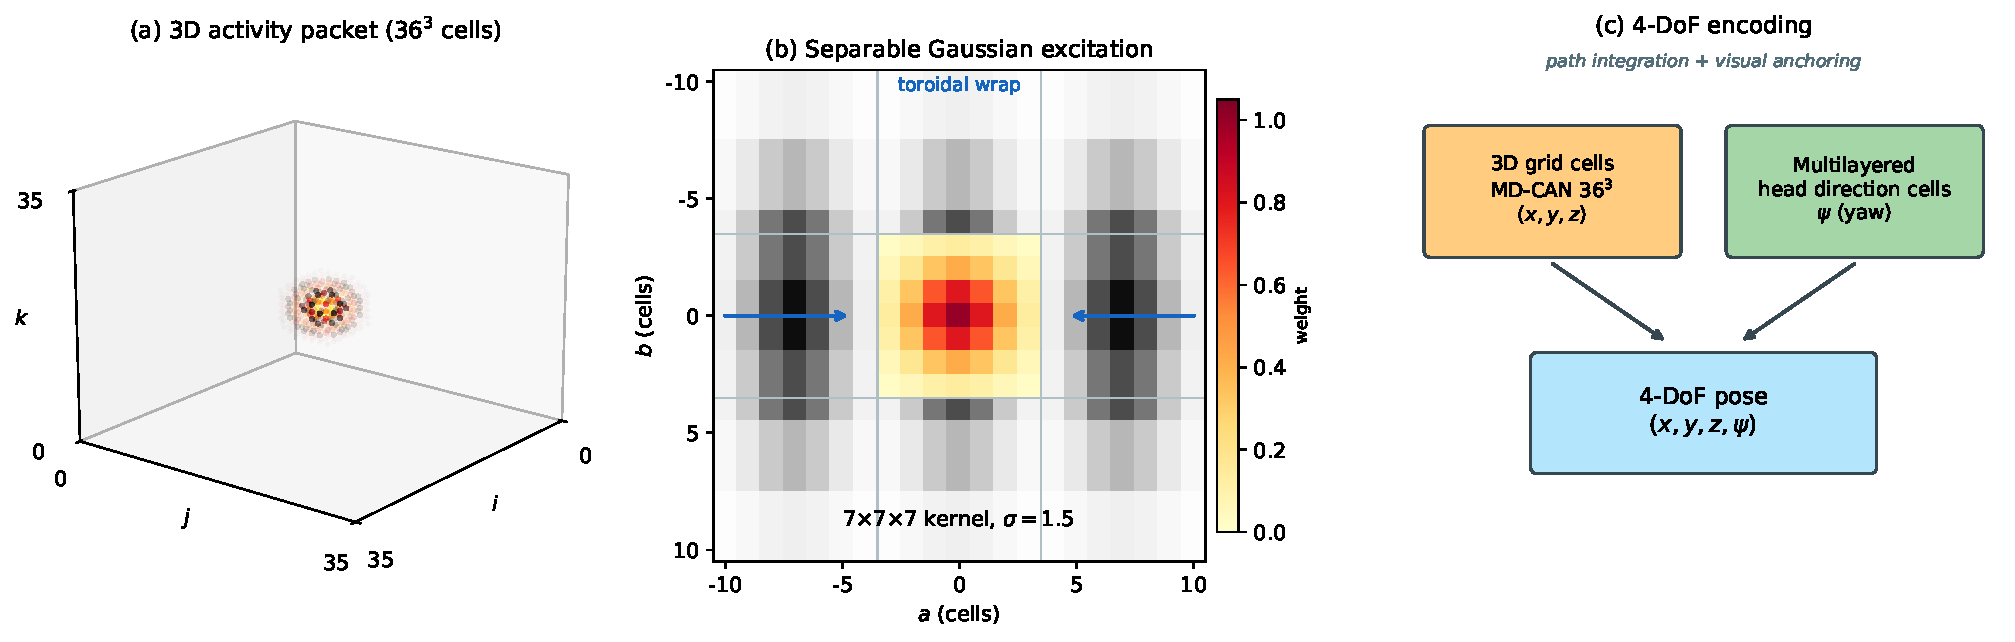
\includegraphics[width=\textwidth]{fig/3d_grid_cell_network.pdf}
    \caption{3D grid cell network. (a) 3D activity packet representing position $(x,y,z)$ through distributed population code. (b) Separable Gaussian excitation kernel ($7\times7\times7$ cells, $\sigma=1.5$ cells per axis) with toroidal wrapping. (c) 4-DoF encoding scheme combining position and heading representations.}
    \label{fig:3D_grid_cell_network}
\end{figure*}

Figure~\ref{fig:3D_grid_cell_network} schematically illustrates: (a) the 3D activity bump at position $(x, y, z)$, represented as isosurfaces to visualize the localized excitation; (b) the separable Gaussian excitation kernel and its toroidal wrapping on the cubic cell lattice; (c) the complete 4-DoF encoding pipeline integrating position and heading representations.

\textbf{Continuous Attractor Dynamics.} The network maintains a localized ``bump'' of activity through three key mechanisms:

\textbf{(1) Local excitation.} Cells excite their neighbors according to a Gaussian connectivity kernel. With a separable kernel
\begin{equation}
    \mathcal{K}^\mathrm{g}_{a,b,c}=\mathcal{N}(a;0,\sigma_x)\mathcal{N}(b;0,\sigma_y)\mathcal{N}(c;0,\sigma_z)
\end{equation}
where $\mathcal{N}(\cdot;\mu,\sigma)$ denotes one-dimensional Gaussian distribution, and $\sigma_x,\sigma_y,\sigma_z$ are spatial kernel widths along three axes.
the excitatory update is:
\begin{equation}
    \Delta A^\mathrm{g}_{i,j,k}=\sum_{p,q,r} A^\mathrm{g}_{p,q,r}\,\mathcal{K}^\mathrm{g}_{\langle i-p\rangle_{N_x},\langle j-q\rangle_{N_y},\langle k-r\rangle_{N_z}}
\end{equation}
where $\langle \cdot \rangle_N$ denotes modulo-$N$ wrapping for periodic boundary conditions. In our implementation $\sigma_x = \sigma_y = \sigma_z = 1.5$ cells with a $7\times7\times7$ kernel.

\textbf{(2) Global inhibition and normalization.} Uniform global inhibition subtracts a fixed threshold $\theta_g$ with rectification, which suppresses weak background activity while preserving the bump:
\begin{equation}
    A^\mathrm{g}_{i,j,k}\leftarrow \big[A^\mathrm{g}_{i,j,k}+\Delta A^\mathrm{g}_{i,j,k}-\theta_g\big]_+,\quad [\cdot]_+ = \max(0, \cdot)
\end{equation}
In our implementation $\theta_g = 2\times10^{-4}$. After inhibition, the activity is $L_1$-normalized:
\begin{equation}
    A^\mathrm{g}\leftarrow \frac{A^\mathrm{g}}{\lVert A^\mathrm{g}\rVert_1}=\frac{A^\mathrm{g}}{\sum_{i,j,k}|A^\mathrm{g}_{i,j,k}|}
\end{equation}
This normalization ensures the activity pattern has unit total mass, making the readout (center of mass) insensitive to overall activity magnitude.

\textbf{(3) Path integration.} The activity bump shifts according to fused velocity cues $\mathbf{v}^\mathrm{f}_t = (v^f_x, v^f_y, v^f_z)$. Index shifts are computed as:
\begin{equation}
    (\Delta i,\Delta j,\Delta k)=\big(\lfloor \gamma_x v^f_x\Delta t\rfloor,\ \lfloor \gamma_y v^f_y\Delta t\rfloor,\ \lfloor \gamma_z v^f_z\Delta t\rfloor\big)
\end{equation}
where $\gamma_x,\gamma_y,\gamma_z$ are metric-to-index gain factors converting physical velocity to network grid shifts.
\begin{equation}
    A^\mathrm{g}_{i,j,k}\leftarrow A^\mathrm{g}_{\langle i-\Delta i\rangle_{N_x},\langle j-\Delta j\rangle_{N_y},\langle k-\Delta k\rangle_{N_z}}
\end{equation}
This discrete shifting operation efficiently implements path integration on the toroidal network topology.

\textbf{Visual Anchoring and Drift Correction.} Pure path integration accumulates drift over time. To prevent unbounded error, the grid cell activity is anchored to visual landmarks through a static, creation-time association: each visual template $m$ records the grid-cell coordinates $(g^x_m,g^y_m,g^z_m)$ and head-direction heading of its creation instant, i.e., the path-integration state at that moment. When template $m$ is matched by a later frame, corrective activity is injected at its recorded coordinates:
\begin{equation}
    \Delta A^\mathrm{g}_{g^x_m,g^y_m,g^z_m} \mathrel{+}= E_0\cdot\frac{30-e^{1.2 d_m}}{30},\qquad d_m\in[0,d_{\max}]
\end{equation}
where $E_0$ is the baseline injection energy and $d_m$ is the template activity level: it is reset to the cap $d_{\max}$ upon each match and decays linearly over time. The injected amplitude grows as a template remains unmatched for longer, from $\approx E_0/3$ at $d_m=d_{\max}$ toward $E_0$ as $d_m\to 0$. This decayed, weak injection is a RatSLAM-style anti-capture design: a single spurious match (e.g., during agent stasis) cannot capture the grid-cell network; a consistent injection from multiple visual templates is required to form an effective anchoring.

We note that in the final system configuration, this template-level injection pathway is deactivated (the deployed visual-template implementation never clears its first-match flag, so the injection condition is never met); visually driven drift correction in the deployed system is carried entirely by the anchoring--re-anchoring mechanism of the experience map.

\textbf{Multilayered Head Direction Cells.} The multilayered head direction cell (HDC) network represents the robot's orientation using a 2D MD-CAN with dimensions $N_\psi \times N_h$ (azimuth bins by height layers). Different height layers allow representation of heading at various vertical positions, supporting 3D operation where orientation may vary with altitude.

\textbf{Network Architecture.} The multilayer head-direction network has activity $\mathbf{A}^\mathrm{h} \in \mathbb{R}^{N_\psi \times N_h}$ (typically $N_\psi = 360$ azimuth bins and $N_h = 5$ height layers). Each cell $(u, h)$ is tuned to azimuth angle $\theta_u = 2\pi u / N_\psi$ and height layer $h$.

\textbf{Attractor Dynamics.} Similar to the grid cell network, the HDC network employs local excitation, global inhibition, and path integration. With a Gaussian kernel $\mathcal{K}^\mathrm{h}$:
\begin{equation}
    \Delta A^\mathrm{h}_{\psi,h}=\sum_{u,v}A^\mathrm{h}_{u,v}\,\mathcal{K}^\mathrm{h}_{\langle \psi-u\rangle_{N_\psi},\langle h-v\rangle_{N_h}}
\end{equation}
followed by fixed-threshold global inhibition ($\theta_h = 2\times10^{-4}$, the same rectify-and-subtract form as above) and $L_1$ normalization:
\begin{equation}
    A^\mathrm{h}\leftarrow \frac{\tilde{A}^\mathrm{h}}{\lVert \tilde{A}^\mathrm{h}\rVert_1},\qquad \tilde{A}^\mathrm{h}=\big[A^\mathrm{h}+\Delta A^\mathrm{h}-\theta_h\big]_+
\end{equation}
Path integration shifts the activity bump according to yaw rate $r^f$ and vertical velocity $v^f_z$:
\begin{equation}
    \Delta\psi=\lfloor \gamma_\psi r^f \Delta t\rfloor,\quad \Delta h=\lfloor \gamma_h v^f_z \Delta t\rfloor
\end{equation}
where $\gamma_\psi$ converts angular velocity to azimuth bins, and $\gamma_h$ maps vertical velocity to height layer shifts.
\textbf{Pose Readout.} The metric pose estimate is decoded from the spatial cell activities via center-of-mass computation (population vector decoding):
\begin{align}
    \hat{\mathbf{p}}_t & = ({\hat x}_t, {\hat y}_t, {\hat z}_t) = \frac{\sum_{i,j,k} \mathbf{c}_{i,j,k} A^\mathrm{g}_{i,j,k,t}}{\sum_{i,j,k} A^\mathrm{g}_{i,j,k,t}}, \quad \mathbf{c}_{i,j,k} = (x_i, y_j, z_k) \\
    \hat{\psi}_t       & = \mathrm{\mathrm{atan2}}\left(\sum_{u,h} A^\mathrm{h}_{u,h,t} \sin\theta_u, \sum_{u,h} A^\mathrm{h}_{u,h,t} \cos\theta_u\right), \quad \theta_u = 2\pi u / N_\psi
\end{align}
This decoding naturally handles the circular topology of orientation (using $\mathrm{\mathrm{atan2}}$ to avoid angle wrapping issues) and provides sub-bin resolution for position through the weighted average.

\textbf{Where the Spatial Layer Sits.} The grid-cell and head-direction layers are not a second estimator. They consume the filtered pose --- frame-to-frame displacement and yaw in EKF-odometry mode --- integrate it into a bump of activity, and expose the resulting spatial code for experience creation, with the head-direction layer supplying the yaw channel of the 4-DoF code. Decoding the bump returns a pose that is used to gate novelty and to define loop constraints, not to correct the filter; the attractor dynamics therefore stabilise the representation rather than revise the estimate. This directionality --- filter, spatial code, constraints, output trajectory --- keeps the layer biologically interpretable without turning it into a competing estimator.

\subsection{Hippocampal Experience Map and Loop Closure}
\label{sec:loop_closure}

In the brain, the hippocampus links place representations into episodic memories of traversed space, and their replay and re-consolidation underpin memory-guided navigation. The multilayered experience map mirrors this organization: it represents 3D spatial experiences as a graph structure, providing a hybrid topological-metric representation that combines the benefits of discrete place-based maps (topological robustness, loop closure) and continuous metric representations (accurate localization).

\textbf{Experience Representation.} Each experience node $\mathcal{E}_i$ encodes a distinct spatial episode comprising the active visual template and descriptor $(VT_i,\,\boldsymbol{\phi}_i\in\mathbb{R}^{192})$, the concurrent spatial-cell codes $\mathbf{P}^{gc}_i=\mathbf{A}^\mathrm{g}_i\in\mathbb{R}^{N_x\times N_y\times N_z}$ and $\mathbf{P}^{hdc}_i=\mathbf{A}^\mathrm{h}_i\in\mathbb{R}^{N_\psi\times N_h}$, the metric pose $(x_i, y_i, z_i, \psi_i)$ decoded from these activities, and the timestamp $t_i$ for temporal ordering.
This rich multimodal encoding enables robust loop closure detection through visual matching while maintaining metric information through the spatial cell codes.

\textbf{Experience Creation and Linking.} As the robot navigates, new experiences are created when the current spatial representation differs sufficiently from all existing experiences. The creation criterion combines visual and spatial cell similarity:
\begin{equation}
    \begin{aligned}
        \text{Create new experience if }\; & d_{cos}(\boldsymbol{\phi}_t, \boldsymbol{\phi}_j) > \tau_{VT} \quad \text{for all } j \in \mathcal{E} \\
                                           & \text{or } \lVert (\hat{x}_t, \hat{y}_t, \hat{z}_t) - (x_j, y_j, z_j) \rVert > d_{thresh}
    \end{aligned}
\end{equation}
where $\tau_{VT} = 0.08$ is the visual template matching threshold and $d_{thresh}$ is a spatial distance threshold (typically 0.5~m).

Consecutive experiences are linked by directed edges encoding the relative pose transition:
\begin{equation}
    \mathbf{T}_{i \to i+1} = (\Delta x, \Delta y, \Delta z, \Delta \psi) = (x_{i+1} - x_i, y_{i+1} - y_i, z_{i+1} - z_i, \psi_{i+1} - \psi_i)
\end{equation}
These edges form the primary topological structure of the experience map graph $\mathcal{G} = (\mathcal{V}, \mathcal{E})$.

\textbf{Loop Closure Detection.} Loop closure is detected when the current visual template matches a previous experience beyond a minimum temporal separation (to avoid trivial closures):
\begin{equation}
    \begin{aligned}
        \text{Loop closure detected if } \exists j:\; & d_{cos}(\boldsymbol{\phi}_t, \boldsymbol{\phi}_j) < \tau_{loop} \\
                                                      & |t - t_j| > T_{min}
    \end{aligned}
\end{equation}
where $\tau_{loop} = 0.05$ (stricter than the template creation threshold to reduce false positives) and $T_{min} = 50$ frames (approximately 5 seconds at 10 Hz).

Upon detecting a loop closure, a loop edge is added to the graph with the pose residual:
\begin{equation}
    \mathbf{T}_{loop} = (\hat{x}_t - x_j, \hat{y}_t - y_j, \hat{z}_t - z_j, \hat{\psi}_t - \psi_j)
\end{equation}
This loop constraint typically violates graph consistency (due to accumulated drift), triggering map relaxation.

\textbf{Map Relaxation.} Map relaxation distributes the loop closure error across all experiences along the loop path to minimize global inconsistency. We employ an iterative relaxation algorithm:

\textbf{Step 1: Identify loop path.} Given a loop closure edge from experience $j$ to experience $t$, identify the sequence of experiences $\mathcal{P} = \{j, j+1, \ldots, t-1, t\}$ along the path.

\textbf{Step 2: Compute pose residual.} The accumulated pose transition along the loop should ideally close (return to the origin):
\begin{equation}
    \mathbf{e}_{loop} = \sum_{k \in \mathcal{P}} \mathbf{T}_{k \to k+1} - \mathbf{T}_{loop}
\end{equation}
where $\mathbf{e}_{loop}$ is accumulated pose drift residual around closed trajectory, and $\mathcal{P}$ denotes ordered experience sequence forming the loop.
\textbf{Step 3: Distribute correction.} Distribute the correction proportionally across the loop experiences:
\begin{equation}
    \mathbf{T}_{k \to k+1} \leftarrow \mathbf{T}_{k \to k+1} - \frac{\mathbf{e}_{loop}}{|\mathcal{P}|}
\end{equation}
This uniform distribution assumes drift accumulates at a constant rate, a reasonable first-order approximation.

\textbf{Step 4: Update experience poses.} Recompute all experience poses by integrating the corrected transitions:
\begin{equation}
    (x_{k+1}, y_{k+1}, z_{k+1}, \psi_{k+1}) = (x_k, y_k, z_k, \psi_k) + \mathbf{T}_{k \to k+1}
\end{equation}

\textbf{Step 5: Re-anchor spatial cells.} Inject the corrected pose $(\hat{x}, \hat{y}, \hat{z}, \hat{\psi})_{corr}$ back into the spatial cell networks by reinitializing the activity bumps at the corrected locations. This ``resets'' the path integration from the corrected reference, preventing error accumulation in subsequent operation.

This relaxation procedure runs iteratively until convergence or a maximum number of iterations, ensuring the experience map remains globally consistent while preserving local metric accuracy.

\textbf{Deployed Loop-Closure Line: Frame-Based Candidates.} The formulation above describes the node-level reference map; every loop result reported in this paper comes from the frame-level line specified here, which instantiates loop-closure detection over \emph{frames} rather than experience nodes: every frame is described by a frozen DINOv2-S global scene embedding $\mathbf{e}_t$, refined by a fine-tuned head trained under the same train-once protocol as the scale branch (simulation data only). A candidate match for the current frame is the historical frame $j^{*} = \arg\max_{j} \cos(\mathbf{e}_t, \mathbf{e}_j)$ restricted to frames whose EKF-odometry arc-length separation exceeds $\mathrm{arc}_{\min}$ (50~m) --- an arc-length criterion replacing the $T_{\min}$ frame gap of the node-level formulation --- which removes trivial self-matches while keeping the search exhaustive over the plausible far-history. This frame-level candidate stage decouples loop detection from experience-node creation and provides dense per-frame evidence to the gate chain.

\textbf{Four-Gate Chain.} A candidate becomes an accepted loop event only if it passes four fixed gates (all thresholds set once across all five scenarios):
\begin{align}
    \mathrm{accept}(t, j^{*}) \iff{}
    & \cos(\mathbf{e}_t, \mathbf{e}_{j^{*}}) \ge \tau
    \;\wedge\; \mathrm{streak}(t, j^{*}) \ge 15 \nonumber\\
    &\;\wedge\; |\Delta\psi_{t j^{*}}| \le 60^{\circ}
    \;\wedge\; \lVert \mathbf{c}_{t j^{*}} \rVert \le 25\,\mathrm{m},
    \label{eq:pr_gates}
\end{align}
with a cumulative correction budget $\sum_i \lVert \mathbf{c}_i \rVert \le 35$~m across the trajectory and deduplication of historical anchors (each past frame anchors at most once). The \emph{similarity gate} ($\tau = 0.94$) is calibrated by a five-scenario sweep: observed false candidates score 0.907--0.935 while strong genuine revisits score $\ge 0.949$. The \emph{persistence gate} ($\ge 15$ consecutive candidate frames, $\pm 10$ tolerance) exploits a structural property of genuine revisits: a vehicle traversing the same street produces a sustained streak of high-similarity frames, whereas perceptual aliasing produces single-frame or short-burst excursions --- this gate is scale-free and transfers across domains unchanged. The \emph{orientation gate} ($60^{\circ}$ heading difference) admits same-direction and reversed re-visits while rejecting geometrically implausible matches. The correction budget bounds the damage of any single wrong acceptance. The chain is deliberately conservative: on KITTI~09 its sole genuine loop lies in the final two frames, where the streak can reach only $2 < 15$ and the gate correctly declines --- releasing it in hindsight would change the error by merely $-0.12$~m --- while the orientation gate rejects that sequence's two high-similarity but geometrically inconsistent candidates (Supplementary Section~S.3). Prefer silence to a wrong re-anchor.

\textbf{Injection.} An accepted event injects a one-shot translation correction $\mathbf{c}_{t j^{*}}$ (step size $\beta = 1.0$) that pulls the current segment toward the matched node's map pose, writes a link edge into the experience graph, and hands the event to the full-Sim(3) re-anchoring operator described below; the corrected segment then enters the drift-field relaxation above.

\textbf{Distributed Closure Drift Field.} Each re-anchoring event (a loop closure or a match to an existing node) resets the incremental dead-reckoning state, so the raw output trajectory contains a discrete correction step of $\mathbf{c}_i$ at frame $f_i$. These steps form an accumulated staircase $\mathbf{C}_{\mathrm{cum}}(f)$ whose discrete jumps are the dominant source of per-frame inconsistency between the experience-map-corrected output and the filtering front-end. We therefore relax each step into a continuous drift field, inspired by slow re-consolidation of spatial memory in the hippocampal--entorhinal system. For every recorded re-anchoring pulse $\mathbf{c}_i$ at frame $f_i$ with $\lVert\mathbf{c}_i\rVert \le C_{\max}$, a raised-cosine ramp of duration $W_i$ is applied:
\begin{equation}
    F_i(f) =
    \begin{cases}
        \tfrac{1}{2}\bigl(1-\cos(\pi (f-f_i)/W_i)\bigr), & f_i \le f < f_i + W_i \\
        1, & f \ge f_i + W_i
    \end{cases}
\end{equation}
and the corrected trajectory is
\begin{equation}
    \hat{\mathbf{p}}(f) = \mathbf{p}_{\mathrm{exp}}(f) + \Bigl(\sum_i F_i(f)\,\mathbf{c}_i \;-\; \sum_{i:\,f_i \le f}\mathbf{c}_i\Bigr),
\end{equation}
so each correction persists (the held level $\mathbf{c}_i$ is retained after the ramp) but its onset is smoothed over $W_i$ frames, and the staircase $\mathbf{C}_{\mathrm{cum}}$ is exactly replaced by the continuous field. Three design choices, validated by offline parameter sweeps on all five outdoor sequences, shape the field:
\begin{itemize}
    \item \textbf{Adaptive relaxation time.} $W_i = \mathrm{clip}(W_0 + W_{\perp}\,\lVert\mathbf{c}_i\rVert,\; W_0,\; W_{\max})$: larger jumps relax more slowly, analogous to the slower re-consolidation of stronger spatial memories and to the longer time constants of grid-cell drift correction.
    \item \textbf{Tail completion.} Each ramp is truncated at the trajectory end ($W_i \leftarrow \min(W_i, f_{\mathrm{end}}-f_i+1)$) so that the drift field is fully relaxed by the final frame, avoiding a half-relaxed ramp that would leave terminal bias.
    \item \textbf{Amplitude gating.} Jumps with $\lVert\mathbf{c}_i\rVert > C_{\max}$ are applied instantaneously and excluded from the field: large corrections correspond to distant true loop closures whose early node positions are trustworthy, whereas small corrections (nearby re-visits, hash collisions) are uncertain and benefit from slow relaxation. Sweeps show that flattening \emph{all} steps degrades accuracy (e.g., Town01: +0.64\% RMSE), while gating yields per-frame RMSE improvements over both the un-relaxed baseline and the EKF front-end on all five sequences.
\end{itemize}
With the EKF-odometry mode ($\mathrm{NLM\_USE\_EKF\_ODO}$) the experience map consumes the fused EKF trajectory as its motion source (frame-to-frame displacement and yaw increments), and new experience nodes are pinned to the EKF map coordinates, so the grid-cell path integrator and the experience graph operate on a common, tightly constrained metric ground truth; the drift field then corrects only the residual re-anchoring steps on top of this unified foundation.

\textbf{Closed-Loop Full-Sim(3) Re-Anchoring.} Each re-anchoring pulse above translates the subsequent trajectory but does not change its global scale or orientation, so the monocular scale ambiguity keeps accumulating between loops. We therefore complement it with a loop-triggered operator: at every accepted loop-closure event at frame $t_{\mathrm{now}}$, a full similarity transform is fitted between the \emph{anchor window} $\mathbf{A}$ (the first $\mathrm{win}$ moving frames of the trajectory, after the static prelude) and the \emph{current window} $\mathbf{C}$ (the $\mathrm{win}$ frames ending at $t_{\mathrm{now}}$, capped by the next event) by a Procrustes fit
\begin{equation}
    \mathbf{A} \approx s\,(\mathbf{C}\mathbf{R}) + \mathbf{t}, \qquad s \in [0.05,\,20],
\end{equation}
with $\mathrm{win} = 250$ frames (self-calibrated by an offline window sweep) and the scale gate rejecting degenerate fits. The entire segment after $t_{\mathrm{now}}$ (up to the next event) is then pulled back into the anchor frame,
\begin{equation}
    \hat{\mathbf{p}}(f) = s\,(\mathbf{p}(f)\mathbf{R}) + \mathbf{t}, \qquad t_{\mathrm{now}} < f < t_{\mathrm{next}},
\end{equation}
applied independently per event on the pre-correction trajectory (non-chained, so one event's refit is not polluted by its predecessor's transform). Because each accepted loop is a genuine re-visit of the same physical location, the re-anchoring is a global consistency correction that uses no ground-truth information; on loop-free routes it is a strict no-op. On a dedicated closed-loop benchmark (an urban route crossing the same road segments at widely separated times), this full-Sim(3) re-anchoring recovers $9\times$ more of the accumulated global drift than the EKF baseline (44.24~m vs 398.05~m, anchored-Sim(3) caliber): the dominant global error accumulated between loops is the monocular scale error, which only the full similarity re-fit removes.
